% \begin{frame}[t]\frametitle{Model Predictive Control: History}
% \begin{columns}
% % --- Left column: meme image ---
% \column{0.4\textwidth}
% \includegraphics[width=\columnwidth]{Figures/memes_mpc.jpg}

% % --- Right column: main image + zoom ---
% \column{0.6\textwidth}
% \begin{tikzpicture}
%   % Main image
%   \node[anchor=south west,inner sep=0] (img) at (0,0) 
%     {\includegraphics[width=0.8\columnwidth]{Figures/mpc_history_0.png}};
  
%   % Coordinate system relative to the image
%   \begin{scope}[x={(img.south east)},y={(img.north west)}]
%     % Region of interest (ROI) -- adjust later
%     \path (0.5,0.8) rectangle (0.25,0.35);

%     % Highlight rectangle
%     \draw[red,thick,rounded corners] (0.41,0.8) rectangle (0.59,0.70);
%     \fill[red,opacity=0.2] (0.41,0.8) rectangle (0.59,0.70);

%     % --- Zoomed inset ---
%     \begin{scope}[xshift=3.5cm,yshift=4cm] % adjust placement
%       \node[draw=red,thick,rounded corners,inner sep=2] (zoom) 
%         {\includegraphics[width=0.4\columnwidth]{Figures/mpc_history_0.png}};
%     \end{scope}

%     % Connect ROI to zoom box
%     \draw[red,thick] (0.59,0.8) -- (zoom.south east);
%     \draw[red,thick] (0.41,0.8) -- (zoom.south west);

%   \end{scope}
% \end{tikzpicture}
% \end{columns}
% \end{frame}
%------------------------------
\begin{frame}[t]\frametitle{History}%Model Predictive Control: 
\begin{columns}
  % --- Left column: meme image ---
  \column{0.4\textwidth}
\only<1>{  \includegraphics[width=\columnwidth]{Figures/memes_mpc.jpg}}
\only<2>{
% \vspace{-1cm}
    \put(00,40){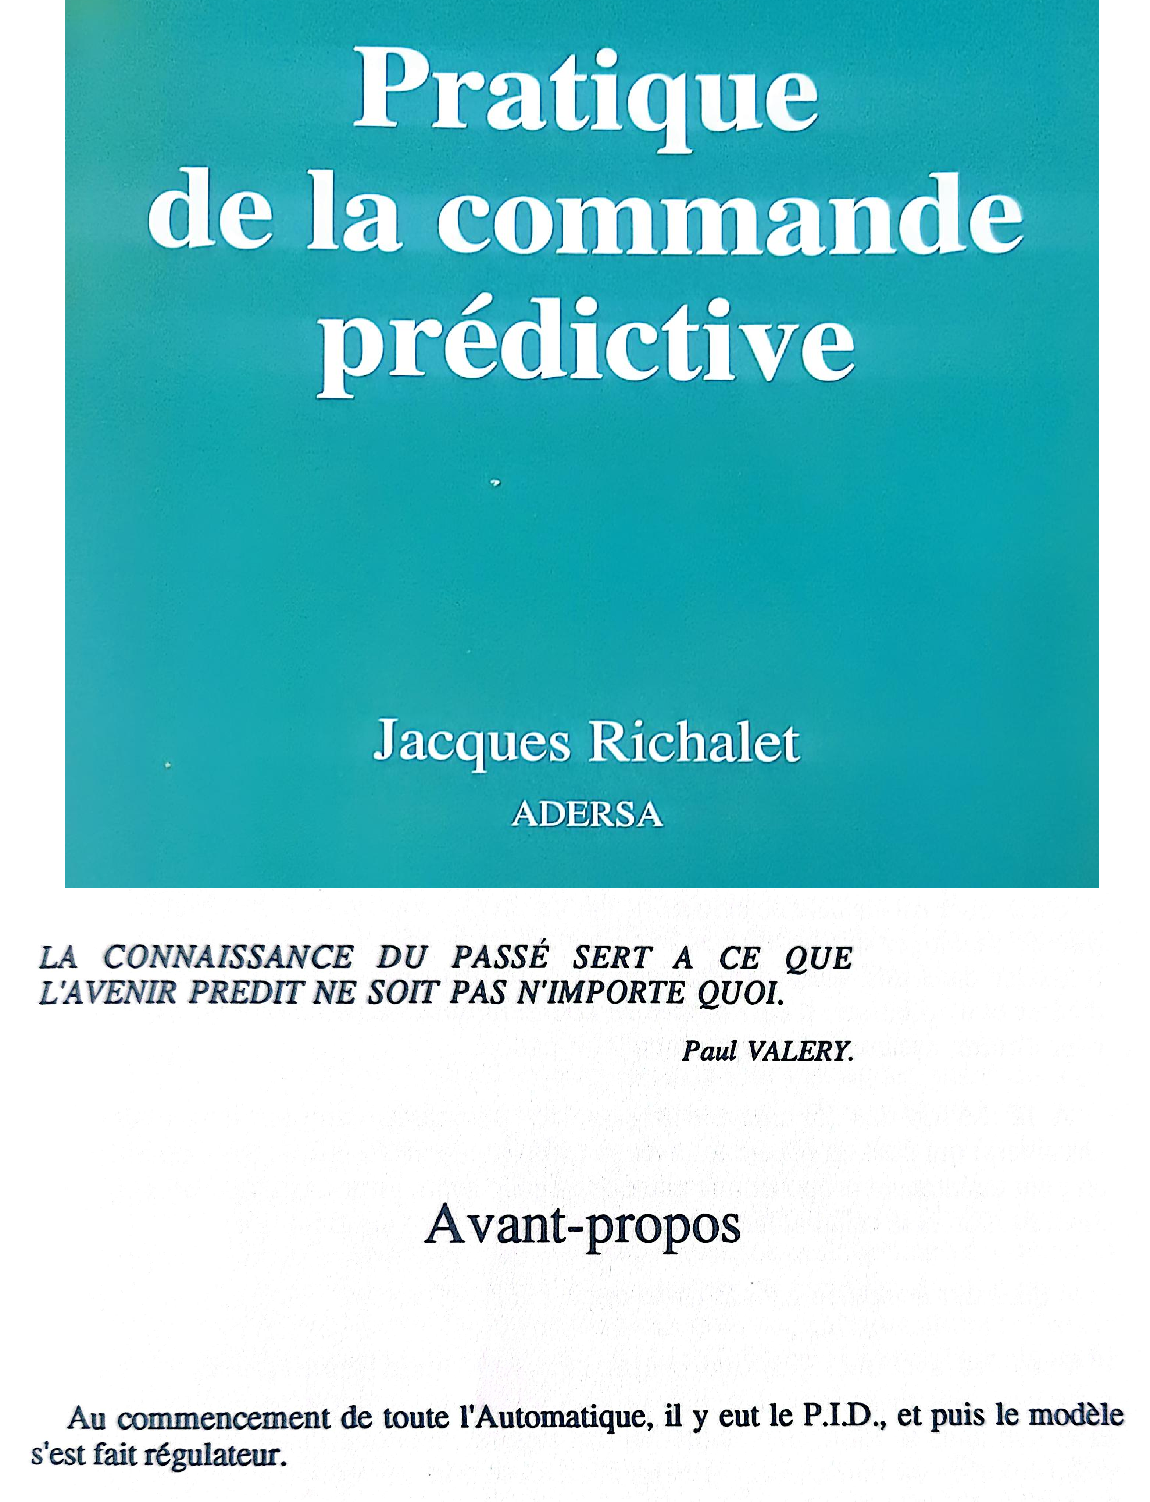
\includegraphics[width=0.8\linewidth]{Figures/richalet_book.pdf}%
    }
% \begin{overpic}[width=0.7\columnwidth]{Figures/mpc_book.pdf}
%   % Position of the overlay (x%, y%)
%   \put(30,40){%
%   }
% \end{overpic}
}

\column{0.6\textwidth}
\only<1>
{
\vspace*{-1cm}
  \begin{block}{Early Form of MPC- Advanced Process Control}
  % \footsizenote
  \small
  The first iterations of what to be known now as MPC, are found in the~\textbf{60s}:
  \begin{itemize}
    \footnotesize
      \item \textbf{Propoi 1963}: It is considered one of the early theoretical proposals that contained the fundamental principles of what would become modern MPC.
      \item \textbf{Rafal, Stevens 1968}: It describes a discrete dynamic optimization algorithm considered a precursor to modern Model Predictive Control (MPC).
      \includegraphics[width=0.6\columnwidth]{Figures/First_papers_on_mpc_0.png}
    \end{itemize}  
  \end{block}
  
}
\only<2>
{
  % \column{0.6\textwidth}

{  \small
    \textbullet Two pioneering research groups in the late 1970s developed the first model predictive Control algorithms for industrial usage.
  \begin{itemize}
    \item ADERSA
    \item American Shell Oil Company (1979-80)
  \end{itemize}}
  \begin{tikzpicture}[spy using outlines={rectangle,thick,red,fill=red,opacity=0.2,
                      lens={scale=2.5}, width=2.8cm, height=1cm, connect spies}]
    % Place main figure
    \node (image) {\includegraphics[width=0.8\columnwidth]{Figures/mpc_history_0.png}};

    % Spy on coordinates (x,y) in the image coordinate system
    % Adjust (x,y) to your region of interest
    \spy on (0.12,0.7) in node [fill=white] at (4,1);
    % \fill[red,opacity=0.2] (0.41,0.8) rectangle (0.59,0.70);

  \end{tikzpicture}
}
\end{columns}
\end{frame}
%------------------------------
\begin{frame}[t]\frametitle{Model Predictive Control: Definition}
\vspace*{-0.5cm}
\begin{columns}
\column{0.4\textwidth}

  \begin{definition}
  \small
An optimization strategy that is based on the systems model.
In other words, having a plant model, allows to run different forecasts forward in time of this model subject to the command { $\mathbf{u}$}, then it optimizes over this latter.
  \end{definition}
\column{0.6\textwidth}
      \begin{figure}[!htb]
        \centering
        % \fontsize{5pt}{5pt}\selectfont
        \fontsize{\dimexpr\linewidth/30}{\dimexpr\linewidth/30}\selectfont
        \def\svgwidth{\textwidth}
        \input{Figures/MPC_graph_theoretical.pdf_tex}
      \end{figure}

  \end{columns}
\end{frame}
\begin{frame}[t]\frametitle{Model Predictive Control: Key concepts}
% \textbullet Linear prediction model
\only<1-3>
{\begin{itemize}
    \item \textbf{Linear prediction model}
\end{itemize}}
\only<1>{
\noindent
\begin{minipage}[t]{0.55\linewidth}
\begin{tcolorbox}[colback=white, colframe=gray!50, left=3mm, right=3mm]
\[
\begin{array}{l}
x_{k+1} = A x_k + B u_k \\
y_k = C x_k
\end{array}
\qquad
\begin{array}{l}
x \in \mathbb{R}^n \\
u \in \mathbb{R}^m \\
y \in \mathbb{R}^p
\end{array}
\]
\end{tcolorbox}
\end{minipage}%
\hfill
\begin{minipage}[t]{0.42\linewidth}
\begin{tcolorbox}[colback=orange!20, colframe=orange!70!black, title=Notation]
\[
\begin{aligned}
x_0 &= x(t) \\
x_k &= x(t+k|t) \\
u_k &= u(t+k|t)
\end{aligned}
\]
\end{tcolorbox}
\end{minipage}
}
% \vspace{2mm}
\only<2-3>{\begin{itemize}
    \item \textbf{Relation between input and states (Integration Scheme)} 
    \only<2>{
    \begin{tcolorbox}[colback=white, colframe=gray!50, left=3mm, right=3mm]
    \[
    x_k = A^k x_0 + \sum_{j=0}^{k-1} A^j B u_{k-1-j}
    \]
    \end{tcolorbox}
    }
    % \item \textbf{Performance index}
\end{itemize}
}
\only<3->{\begin{itemize}
    \item \textbf{Performance index}
\end{itemize}
\begin{tcolorbox}[colback=white, colframe=gray!50]
% \only<4>{\tiny}
\[
J(z,x_0) = x_N' P x_N + \sum_{k=0}^{N-1} \left( x_k' Q x_k + u_k' R u_k \right)
\]
\vspace*{-0.5cm}
\only<3>{\[
\begin{aligned}
R &= R' \succ 0, & Q &= Q' \succeq 0, & P &= P' \succeq 0,& 
z &= 
\begin{bmatrix}
u_0 \\ u_1 \\ \vdots \\ u_{N-1}
\end{bmatrix}
\end{aligned}
\]}
\end{tcolorbox}
}
\only<4>{
\begin{itemize}
    \item \textbf{Goal:} find the sequence \(z^*\) that minimizes \(J(z,x_0)\), 
    i.e. steers the state \(x\) to the origin optimally.
\end{itemize}
}
% \tracingall
\end{frame}
\begin{frame}[t]\frametitle{Model Predictive Control}
\vspace*{-0.5cm}
% \small 
\only<1>{
\textbullet The cost function can be re-written after few adjustments as follows:
% \end{frame}
% \begin{frame}{Condensed Quadratic Cost in MPC}

\small
\begin{tcolorbox}[colback=white, colframe=gray!50, title={Stage-wise Cost Expansion}]
\[
J(z, x_0) = x_0' Q x_0 + 
\begin{bmatrix}
x_1 \\ x_2 \\ \vdots \\ x_N
\end{bmatrix}^{\!\!\top}
\bar{Q}
\begin{bmatrix}
x_1 \\ x_2 \\ \vdots \\ x_N
\end{bmatrix}
+
\begin{bmatrix}
u_0 \\ u_1 \\ \vdots \\ u_{N-1}
\end{bmatrix}^{\!\!\top}
\bar{R}
\begin{bmatrix}
u_0 \\ u_1 \\ \vdots \\ u_{N-1}
\end{bmatrix}
\]
where
\[
\bar{Q} =
\begin{bmatrix}
Q & 0 & \cdots & 0 \\
0 & Q & \cdots & 0 \\
\vdots & \vdots & \ddots & \vdots \\
0 & 0 & \cdots & P
\end{bmatrix}, \quad
\bar{R} =
\begin{bmatrix}
R & 0 & \cdots & 0 \\
0 & R & \cdots & 0 \\
\vdots & \vdots & \ddots & \vdots \\
0 & 0 & \cdots & R
\end{bmatrix}.
\]
\end{tcolorbox}
}
% \vspace{2mm}
\only<2>{
\begin{tcolorbox}[colback=orange!10, colframe=orange!70!black, title={Condensed Form}]
\[
\begin{bmatrix}
x_1 \\ x_2 \\ \vdots \\ x_N
\end{bmatrix}
= 
\underbrace{
\begin{bmatrix}
B & 0 & \cdots & 0 \\
AB & B & \cdots & 0 \\
\vdots & \vdots & \ddots & \vdots \\
A^{N-1}B & A^{N-2}B & \cdots & B
\end{bmatrix}
}_{\displaystyle \bar{S}}
\begin{bmatrix}
u_0 \\ u_1 \\ \vdots \\ u_{N-1}
\end{bmatrix}
+
\underbrace{
\begin{bmatrix}
A \\ A^2 \\ \vdots \\ A^N
\end{bmatrix}
}_{\displaystyle \bar{T}}
x_0
\]
\[
\Rightarrow \quad
J(z, x_0)
= (\,\bar{S}z + \bar{T}x_0\,)^{\!\top} 
\bar{Q}
(\,\bar{S}z + \bar{T}x_0\,)
+ z^{\top} \bar{R} z + x_0^{\top} Q x_0
\]
\end{tcolorbox}
}
% \vspace{1mm}
\only<3>{
\begin{block}{Compact Quadratic Form}
\small
\[
J(z, x_0) = 
\frac{1}{2} z^{\top} \underbrace{(2(\bar{R} + \bar{S}^{\top}\bar{Q}\bar{S}))}_{H} z
+ \underbrace{x_0^{\top}(\bar{T}^{\top}\bar{Q}\bar{S})}_{F^{\top}} z
+ \frac{1}{2} x_0^{\top} \underbrace{(2(Q + \bar{T}^{\top}\bar{Q}\bar{T}))}_{Y} x_0
\]
\end{block}
\begin{tcolorbox}[colback=red!10, colframe=orange!70!black, title={}]
\[
J(z, x_0) = 
\frac{1}{2} z^{\top} H z
+ {F^{\top}} z
+ \frac{1}{2} x_0^{\top} Y x_0 ,  \quad z = 
\begin{bmatrix}
u_0 \\ u_1 \\ \vdots \\ u_{N-1}
\end{bmatrix}
\]
\end{tcolorbox}
}
\end{frame}
\begin{frame}[t]\frametitle{Model Predictive Control}
\vspace*{-0.5cm}
\only<1>
{
  \textbullet In the \textbf{Unconstrained Case}:\\

  The optimum is obtained by
  \[
    \nabla_z J(z, x_0) = Hz+Fx_0 = 0 
  \]
If considered at each time step $t$:
\[
   z^* = -H^{-1}Fx(t)
\]
\begin{tcolorbox}[colback=red!10, colframe=orange!70!black, title={}]
\centering
Unconstrained linear MPC $\equiv$ Linear state-feedback
\end{tcolorbox}
}
\only<2->
{
    \textbullet In the \textbf{Constrained Case}:\\
 \only<2>{     We introduce the following constraints:
\[
\left\{
\begin{aligned}
y_{\min} &\le y(t) \le y_{\max}, \\
u_{\min} &\le u(t) \le u_{\max},
\end{aligned}
\right.
\qquad
\begin{aligned}
y_{\min},\, y_{\max} &\in \mathbb{R}^p,\\
u_{\min},\, u_{\max} &\in \mathbb{R}^m
\end{aligned}
\]}

\only<2>
{
\textbullet The constrained problem can be then expressed as:
\vspace*{-1.0cm}
\begin{center}
  
% \begin{tcolorbox}[colback=white, colframe=gray!50, title={}]
\centering
\begin{align*}
J(x_0) = 
\frac{1}{2} x_0^{\top} Y x_0
+ 
% \alert<2>{\min_{z}}
% \left(
&\frac{1}{2} z^{\top} H z
+ x_0^{\top} F^{\top} z
% \right) &
\\%[2mm]
\text{s.t.} \quad
& G z \leq W + S x_0 &
\end{align*}
% \end{tcolorbox}
\end{center}


}
    \begin{columns}
    \column{0.6\textwidth}

\only<3>
{    
\begin{flalign*}
J(x_0) = 
\frac{1}{2} x_0^{\top} Y x_0
+\alert<3>{
\min_{z}}
% \left(
&\alert<3>{\frac{1}{2} z^{\top} H z
+ x_0^{\top} F^{\top} z}
% \right) &
\\%[2mm]
\text{s.t.} \quad
&\alert<3>{ G z \leq W + S x_0} &
\end{flalign*}
}
      \column{0.5\textwidth}

\only<3>{
\begin{picture}(30,0)
  \put(20,00){\makebox(0,0)[l]{\textcolor{red}{Quadratic objective}}}
  \put(20,-25){\makebox(0,0)[l]{\textcolor{red}{Linear constraint}}}
\end{picture}
}
\end{columns}
\only<3>
{\vspace*{0.5cm}
\textbullet \textcolor{red}{ It has the QP that we have seen !!}}
}
\end{frame}
%%============================================================%%
\begin{frame}[t]{Model Predictive Control}
  \begin{enumerate}
    \item Uses models explicitly to predict future system behavior
    \item Constraints on inputs, outputs and states are respected
    \item Control sequence is determined by solving an optimization problem each sample 
    \item Combined with state estimation
  \end{enumerate}
\end{frame}

\begin{frame}[t]\frametitle{Model Predictive Control vs LQR}
\vspace*{-0.5cm}

\only<1>{\begin{columns}
\column{0.5\textwidth}

\begin{block}{MPC}
\small 
\begin{itemize}
  \item  Optimizes repeatedly over a finite, receding horizon.
  \item Handles nonlinear models and hard constraints.
  \item Provides flexibility and locally optimal performance but may be sub-optimal overall.
  \item Stability and convergence are not guaranteed without careful problem formulation.
\end{itemize}
\end{block}

\column{0.5\textwidth}
\begin{block}{LQR}
\small 
\begin{itemize}
  \item Optimizes over the entire infinite horizon.
  \item Produces a single fixed control law (state feedback).
  \item Strong global stability but limited to linear systems and no hard constraints.
  \item Performance degrades when the system moves far from the linearized operating point.
\end{itemize}
\end{block}
\end{columns}}

\only<2>{
    \begin{tcolorbox}[colback=green!5!white, colframe=green!75!black, title=One key aspect]
 Both are optimal control methods but differ in how they set up and solve optimization problems.
    \end{tcolorbox}
        \begin{tcolorbox}[colback=green!5!white, colframe=green!75!black, title=Key trade-off:]
        \begin{itemize}
          \item LQR → strong stability, simple, but limited in handling constraints/nonlinearities.
          \item MPC → more versatile, adaptive, and constraint-aware, but computationally demanding and not always globally optimal.
        \end{itemize}
    \end{tcolorbox}
}
\end{frame}
\begin{frame}[t]\frametitle{Model Predictive Control-Example~{\tiny\cite{Haber2023MPC}}}


\end{frame}
\begin{frame}[t]{Model Predictive Control}
  \centering
\embedvideo*{\includegraphics[width=0.8\textwidth]{MPC_Collaborative_ROB.png}}{Figures/mpc_payload_Rob_colaboration_c.mp4}[autoplay=false,showGUI=true]
\end{frame}